%me=0 student solutions (ps file), me=1 - my solutions (sol file), me=2 - assignment (hw file)
\def\me{0}
\def\num{9}  %homework number
\def\due{Tuesday, November 24}  %due date
\def\course{CSCI-GA.1170-001/002 Fundamental Algorithms} %course name, changed only once
\def\name{GOWTHAM GOLI (N17656180)}   %student changes (instructor keeps!)
%
\iffalse
INSTRUCTIONS: replace # by the homework number.
(if this is not ps#.tex, use the right file name)

  Clip out the ********* INSERT HERE ********* bits below and insert
appropriate TeX code.  Once you are done with your file, run

  ``latex ps#.tex''

from a UNIX prompt.  If your LaTeX code is clean, the latex will exit
back to a prompt.  To see intermediate results, type

  ``xdvi ps#.dvi'' (from UNIX prompt)
  ``yap ps#.dvi'' (if using MikTex in Windows)

after compilation. Once you are done, run

  ``dvips ps#.dvi''

which should print your file to the nearest																																															`			 printer.  There will be
residual files called ps#.log, ps#.aux, and ps#.dvi.  All these can be
deleted, but do not delete ps1.tex. To generate postscript file ps#.ps,
run

  ``dvips -o ps#.ps ps#.dvi''

I assume you know how to print .ps files (``lpr -Pprinter ps#.ps'')
\fi
%
\documentclass[11pt]{article}
\usepackage{amsfonts}
\usepackage{latexsym}
\usepackage[lined,boxed,linesnumbered]{algorithm2e}
\usepackage{amsmath}
\usepackage{amsthm}
\usepackage{array}
\usepackage{amssymb}
\usepackage{amsthm}
\usepackage{epsfig}
\usepackage{psfrag}
\usepackage{color}
\usepackage{tikz}
\usepackage{enumerate}
\usetikzlibrary{calc,trees,positioning,arrows,fit,shapes,calc}
\usetikzlibrary{trees}
\usepackage{mathtools}
\usepackage{float}
\setlength{\oddsidemargin}{.0in}
\setlength{\evensidemargin}{.0in}
\setlength{\textwidth}{6.5in}
\setlength{\topmargin}{-0.4in}
\setlength{\textheight}{8.5in}

\newcommand{\handout}[5]{
   \renewcommand{\thepage}{#1, Page \arabic{page}}
   \noindent
   \begin{center}
   \framebox{
      \vbox{
    \hbox to 5.78in { {\bf \course} \hfill #2 }
       \vspace{4mm}
       \hbox to 5.78in { {\Large \hfill #5  \hfill} }
       \vspace{2mm}
       \hbox to 5.78in { {\it #3 \hfill #4} }
      }
   }
   \end{center}
   \vspace*{4mm}
}

\newcounter{pppp}
\newcommand{\prob}{\arabic{pppp}}  %problem number
\newcommand{\increase}{\addtocounter{pppp}{1}}  %problem number

%first argument desription, second number of points
\newcommand{\newproblem}[2]{
\ifnum\me=0
\ifnum\prob>0 \newpage \fi
\increase
\setcounter{page}{1}
\handout{\name, Homework \num, Problem \arabic{pppp}}{\today}{Name: \name}{Due:
\due}{Solutions to Problem \prob\ of Homework \num\ (#2)}
\else
\increase
\section*{Problem \num-\prob~(#1) \hfill {#2}}
\fi
}

%\newcommand{\newproblem}[2]{\increase
%\section*{Problem \num-\prob~(#1) \hfill {#2}}
%}

\def\squarebox#1{\hbox to #1{\hfill\vbox to #1{\vfill}}}
\def\qed{\hspace*{\fill}
        \vbox{\hrule\hbox{\vrule\squarebox{.667em}\vrule}\hrule}}
\newenvironment{solution}{\begin{trivlist}\item[]{\bf Solution:}}
                      {\qed \end{trivlist}}
\newenvironment{solsketch}{\begin{trivlist}\item[]{\bf Solution Sketch:}}
                      {\qed \end{trivlist}}
\newenvironment{code}{\begin{tabbing}
12345\=12345\=12345\=12345\=12345\=12345\=12345\=12345\= \kill }
{\end{tabbing}}

%%%%%\newcommand{\eqref}[1]{Equation~(\ref{eq:#1})}

\newcommand{\hint}[1]{({\bf Hint}: {#1})}
%Put more macros here, as needed.
\newcommand{\room}{\medskip\ni}
\newcommand{\brak}[1]{\langle #1 \rangle}
\newcommand{\bit}[1]{\{0,1\}^{#1}}
\newcommand{\zo}{\{0,1\}}
\newcommand{\C}{{\cal C}}

\newcommand{\nin}{\not\in}
\newcommand{\set}[1]{\{#1\}}
\renewcommand{\ni}{\noindent}
\renewcommand{\gets}{\leftarrow}
\renewcommand{\to}{\rightarrow}
\newcommand{\assign}{:=}
\newcommand{\cT}{\mathcal{T}}

\newcommand{\AND}{\wedge}
\newcommand{\OR}{\vee}

\newcommand{\Forr}{\mbox{\bf For }}
\newcommand{\To}{\mbox{\bf to }}
\newcommand{\Do}{\mbox{\bf Do }}
\newcommand{\Ifi}{\mbox{\bf If }}
\newcommand{\Then}{\mbox{\bf Then }}
\newcommand{\Elsen}{\mbox{\bf Else }}
\newcommand{\Whilee}{\mbox{\bf While }}
\newcommand{\Repeatt}{\mbox{\bf Repeat }}
\newcommand{\Until}{\mbox{\bf Until }}
\newcommand{\Returnn}{\mbox{\bf Return }}
\newcommand{\Swap}{\mbox{\bf Swap }}

\begin{document}

\ifnum\me=0
%\handout{PS\num}{\today}{Name: **** INSERT YOU NAME HERE ****}{Due:
%\due}{Solutions to Problem Set \num}
%
%I collaborated with *********** INSERT COLLABORATORS HERE (INDICATING
%SPECIFIC PROBLEMS) *************.
\fi
\ifnum\me=1
\handout{PS\num}{\today}{Name: Yevgeniy Dodis}{Due: \due}{Solution
{\em Sketches} to Problem Set \num}
\fi
\ifnum\me=2
\handout{PS\num}{\today}{Lecturer: Yevgeniy Dodis}{Due: \due}{Problem
Set \num}
\fi


\newproblem{Shortest Duration}{10 +(6) points}



Consider the following greedy algorithm for the {\sc
Activity-Selection} problem. Select the activity $a_i$ with the
shortest duration $d_i = f_i-s_i$. Commit to scheduling $a_i$. Let
$S_i'$ consist of all activities $a_j$ which do not overlap with
$a_i$: namely, either $f_j\le s_i$ or $f_i\le s_j$. Recursively solve
{\sc Activity-Selection} on $S_i'$, scheduling the resulting
activities together with $a_i$.

\begin{itemize}

\item[(a)] (2 pts) Give a simple example of the input where the proposed
greedy algorithm fails to compute the correct optimal solution.

\ifnum\me<2
\begin{solution}

Consider the following activities, $a_1, a_2$ and $a_3$ such that $(s_1,f_1) = (1,5), (s_2,f_2) = (4,7)$ and $(s_3,f_3) = (6,9)$. By using the above greedy algorithm, the activity selected will be $a_2$ i.e the activity with the shortest duration and $a_1, a_3$ will be excluded as they overlap with $a_2$. Thus the output of the suggested greedy algorithm will be $a_2$. But clearly, the optimal solution is to select the activities $a_1$ and $a_3$. Therefore the proposed greedy algorithm fails to compute the optimal solution
\end{solution}
\fi

\item[(b)] (4 pts) Consider the following attempt to nevertheless justify the
correctness of this algorithm using the ``Greedy Always Ahead''
method. Given a solution $Z$, let $F_i(Z)$ be the sum of the $i$
shortest activities scheduled by $Z$, and $\infty$ if $|Z|<i$. Try to
tell exactly where the claim ``For any $i$ and $Z$, $F_i(Z)\ge
F_i(greedy)$'' fails. Is is base of induction? Or, if in the inductive
step, for what smallest $i$ does the transition from $i$ to $i+1$
fails? Justify your answer.

\ifnum\me<2
\begin{solution}

\textbf{Base Case}

For $i=1$, The greedy strategy chooses the activity of the shortest duration. Hence $F_1(greedy)$ will be lesser than $F_1$ of any other feasible solution $\implies F_1(greedy) \leq F_1(Z)$. Therefore the base case is true

\textbf{Induction Hypothesis}

Assume that $F_i(greedy) \leq F_i(Z) \,\,\,\, \forall i \leq r$

\textbf{Inductive Step}

Let the activities that the greedy strategy selects are $i_1, \ldots, i_r,i_{r+1}$ and the activities that $Z$ selects are $j_1, \ldots, j_r,j_{r+1}$ We need to prove that $F_{r+1}(greedy) \leq F_{r+1}(Z)$

 Let us assume that $F_{r+1}(greedy) > F_{r+1}(Z)$. From the induction hypothesis, we know that $F_r(greedy) \leq F_r(Z)$. Therefore for $F_{r+1}(greedy) > F_{r+1}(Z)$ to happen it must be the case that $d_{i_{r+1}} > d_{j_{r+1}}$. Also $d_{i_{r+1}} > d_{i_r}$. However we cannot make a comparison between $d_{i_r}$ and $d_{j_{r+1}}$.
 
 If $d_{i_r} < d_{j_{r+1}} \implies d_{i_r} < d_{j_{r+1}} < d_{i_{r+1}} $ then the greedy strategy would have selected $j_{r+1}$ instead of $i_{r+1}$ thus contradicting our assumption. Therefore, $F_{r+1}(greedy) \leq F_{r+1}(Z)$. 
 
 Else If $d_{j_{r+1}} < d_{i_r} \implies d_{j_{r+1}} < d_{i_r} < d_{i_{r+1}}  $ then $j_{r+1}$ would have already been selected by the greedy strategy i.e $j_{r+1} \in \{i_1, \ldots i_r\}$ thus our assumption might indeed be true. Therefore, $F_{r+1}(greedy) > F_{r+1}(Z)$
 
 Also if greedy algorithm schedules $k$ activities and $Z$ schedules $m$ activities where $m > k$ then if the given condition were true it would fail from $k$ to $k+1$ as $F_{k+1}(greedy) = \infty$

\end{solution}
\fi

\item[(c)] (4 pts) Consider the following alternative attempt to justify the
correctness of this algorithm using the ``Local Swap''
method. Given a solution $Z$, try to argue that it is always safe to
substitute one activity in $Z$ by the first activity of the greedy
algorithm, and then argue that the resulting recursive subproblems
are the same for the ``perturbed'' opt and the greedy. Where does your
argument run into problem? Is it the swap, or the recursive
subproblem part?

\ifnum\me<2
\begin{solution}

Let $a$ be the activity of shortest duration in the given set of activities and $S$ be the set of all the activities that overlap with $a$.

 Let the activities scheduled by $Z$ be $OPT = \{a_{j_1}, \ldots, a_{j_k}, \ldots, a_{j_m}\}$ and $OPT^*$ be the set of activities obtained after substituting some activity in $OPT$ by $a$.  Now we have two cases
 
 If $OPT$ already contains $a$ in it, then we could simply replace the existing $a$ with $a$. In this case, $OPT^* = OPT$. But if we substitute some $a_k$ by $a$, we have two $a$'s in $OPT^*$. So exclude one of the duplicates then $|OPT^*| = |OPT|-1$ . Therefore, this is not an optimal solution anymore.
 
 If $OPT$ doesn't contain $a$ in it and it has one or more non-overlapping activities from the set $S$. Now  replace some activity $a_k$ in $OPT$ with $a$. Now $OPT^*$ has some overlapping activities in it. So eliminate all those activites that overlap with $a$ from $OPT^*$. So $|OPT^*| < |OPT|$. Therefore, this is not an optimal solution anymore. 
 
 Therefore the argument runs into a problem when we swap some activity in $Z$ with the first activity of the greedy algorithm
\end{solution}
\fi

\item[(d)] ({\bf Extra credit}) (6 pts) Let $t_{opt}$ be the size of the
optimum solution and $t_{bogus}$ be the size returned by the bogus
greedy algorithm discussed. Argue that $t_{bogus}\ge t_{opt}/2$.  To
do this, argue that the first activity $a$ scheduled by the bogus
greedy algorithm overlaps {\em at least} one and {\em at most} two
activities scheduled by the correct optimum algorithm.

In case it overlaps two activities $a_1$ and $a_2$, argue that the
recursive subproblem resulting from scheduling $a$ has the optimum
value at least as large as the one resulting from excluding $a_1$ and
$a_2$ from opt. (Then use induction on the size of $t_{opt}$.)

In the the case of only one activity $a_1$, argue that you can find
at most one more activity $a_2$ in opt such that the recursive
subproblem resulting from scheduling $a$ has the optimum value at
least as large as the one resulting from excluding $a_1$ and $a_2$
from opt. (Then use induction on the size of $t_{opt}$.) How to you
find $a_2$ if you need it? (This is tricky.)

\ifnum\me<2
\begin{solution}

\end{solution}
\fi

\end{itemize}


\newproblem{Listening to CDs}{12 points}



You have $n$ CDs in your library labeled $1,\ldots, n$. You would
like to arrange them on your CD rack in linear order $\pi(1),\ldots,
\pi(n)$, according to some permutation $\pi$ on $n$ numbers. After
such an arrangement is finalized, the cost to access CD $i$ is equal
to $\pi(i)$, as you need to scan through the first $\pi(i)$ CDs until
CD $i$ is found. Given a sequence of $k$ CD requests $r_1,\ldots,
r_k\in \{1\ldots n\}$, your job is to figure out the permutation $\pi$
(i.e., an array $A$ such that $A[i] = \pi(i)$) having the {\em
smallest total access cost} $\sum_{j=1}^k \pi(r_j)$. 

\begin{itemize}
\item[(a)] (4 pts) Describe in English a greedy algorithm for this problem. 
\ifnum\me<2
\begin{solution}

Greedy strategy is to pick that CD $r_j$ that is most frequently used and place it on the top of the stack i.e assign corresponding $\pi(r_j)$ to be the least
\end{solution}
\fi

\item[(b)] (4 pts) Prove the correctness of your algorithm using the local-swap argument.
\ifnum\me<2
\begin{solution}

Let the greedy algorithm algorithm $G$ outputs the permutation $\pi^G$ and the optimal algorithm $Z$ outputs the permutation $\pi^Z$. Let $r_m$ be the CD with maximum number of requests then the greedy algorithm sets $\pi^G_{r_m}$ to 1. Now there is some CD in $\pi^Z$ whose value is set to 1 by $Z$ i.e $\pi^Z_{r_p} = \pi^G_{r_m} =1$. Now substitute $\pi^Z_{r_m}$ with $\pi^G_{r_m}$ then the resulting permutation will have two 1's in it. So substitute  $\pi^Z_{r_p} (=1)$ with the old value of $\pi^Z_{r_m}$. Let the resulting permutation be some $\pi^{Z^*}$. Then $\pi^{Z^*}$ still remains to be optimal as clearly $\sum_{j=1}^{k} \pi^{Z^*}(r_j) \leq \sum_{j=1}^{k} \pi^{Z}(r_j) $. 
Therefore, the \textbf{Lemma} is, In the optimal solution the value of $\pi$ for the CD with maximum number of requests is set to 1

\textbf{Theorem} If $\pi^Z = \pi_{r_m}, \pi^{Z`}$, where $\pi_{r_m} = 1$ i.e $r_m$ is the CD with maximum number of requests and $\pi^{Z`}$ is the optimal permutations of all the CDs starting from 2 i.e excluding $r_m$ then we need to prove that $\pi_z$ is also optimal.

\textbf{Proof} From the above Lemma we know that the optimal solution sets $\pi_{r_m}$ to 1 i.e the CD with maximum number of requests is at the top of the stack so it means that $\pi^Z$ might be an optimal solution. To show that it is indeed an optimal solution we need to prove that  $\sum_{j=1}^{k} \pi^{Z}(r_j) \leq \sum_{j=1}^{k} \pi^{Z^*}(r_j) $.

Let $\pi^{Z^*} = \pi_{r_m}, \pi^{Z^{**}}$ then as $Z^`$ is optimal $\sum \pi^{Z`} \leq \sum \pi^{Z^{**}} = \sum_{j=1}^{k} \pi^{Z*}-\pi_{r_m}$

$\implies \sum_{j=1}^{k} \pi^{Z}(r_j) = \pi_{r_m} + \sum \pi^{Z`} \leq \pi_{r_m} +\sum_{j=1}^{k} \pi^{Z*}-\pi{r_m} \leq \sum_{j=1}^{k} \pi^{Z*} $

Therefore, $\pi^Z$ is an optimal solution. Hence the proposed greedy algorithm is correct
\end{solution}
\fi


\item[(c)] (4 pts) Write the pseudocode for implementation which runs in time $O(n+k)$.
(Hint: At some point use counting sort.) 
\ifnum\me<2
\begin{solution}

\begin{algorithm*}[H]
\TitleOfAlgo{{\sc ArrangeCDs}$(n, r_1, \ldots, r_k)$}

$freq \leftarrow$ {\sc NewArray}$(n)$\\ 
$freq \leftarrow 0$\\
\For{i $\leftarrow$ 1 to k}{
	$freq[r_i] \leftarrow freq[r_i]+1$
}
$CD \leftarrow$ {\sc NewArrayTuples}$(n)$\\
\For{i $\leftarrow$ 1 to n}{
	$CD(i) \leftarrow (i, freq[i]))$
}
\sc{DescendingCountingSort\_Tuples}$(CD)$\\
$counter \leftarrow 1$\\
\For{i $\leftarrow$ 1 to n}{
	$\pi[CD[i](1)] \leftarrow counter$\\
	$counter \leftarrow counter+1$
}

\Returnn $\pi$

\caption{Greedy algorithm to minimize the total access cost of CDs in $O(n+k)$ time }
\end{algorithm*}

In the above pseudocode $freq$ is an array such that $freq(i)$ maintains the frequency of the CD $i$'s requests. This step takes $O(n)$ time.

 $CD$ is an array of tuples such that $CD(i)$ stores the tuple $(i, freq(i))$. Therefore creating this list of tuples $CD$ takes $O(n)$ time. 
 
 Now that we have a list of CDs we need to sort them using their frequencies. {\sc DescendingCountingSort\_Tuples} is a variant of Counting Sort that sorts a list of tuples in descending order based on the second element of the tuple i.e it sorts all the CDs based on their request frequencies. The frequency of the CD requests range between 0 to $k$ and there are total $n$ number of CDs. Therefore this step takes $O(n+k)$ time
 
 Now we have a list of CDs sorted in a decreasing order based on their frequencies. The last $for$ loop iterates through these sorted CDs and assigns them the value of $\pi$ in an increasing order. This step takes $O(n)$ time. Therefore the total running time of the algorithm is $O(n+k)$

\end{solution}
\fi

\end{itemize}








\newproblem{Arithmetic vs. Geometric}{8 points}

Design optimal Huffman codes for the following frequencies
$f_0,\ldots, f_7$. In each case, draw the Huffman tree incrementally,
until you arrive at your final solution. After you finish, which
Huffman code is more ``balanced'': ``arithmetic'' or ``geometric''?

\begin{itemize}
\item[(a)] (4 pts) Arithmetic: $f_i = 10 + i$, for $i=0\ldots 7$.

\ifnum\me<2
\begin{solution}
\begin{figure}[H]
	\centering
	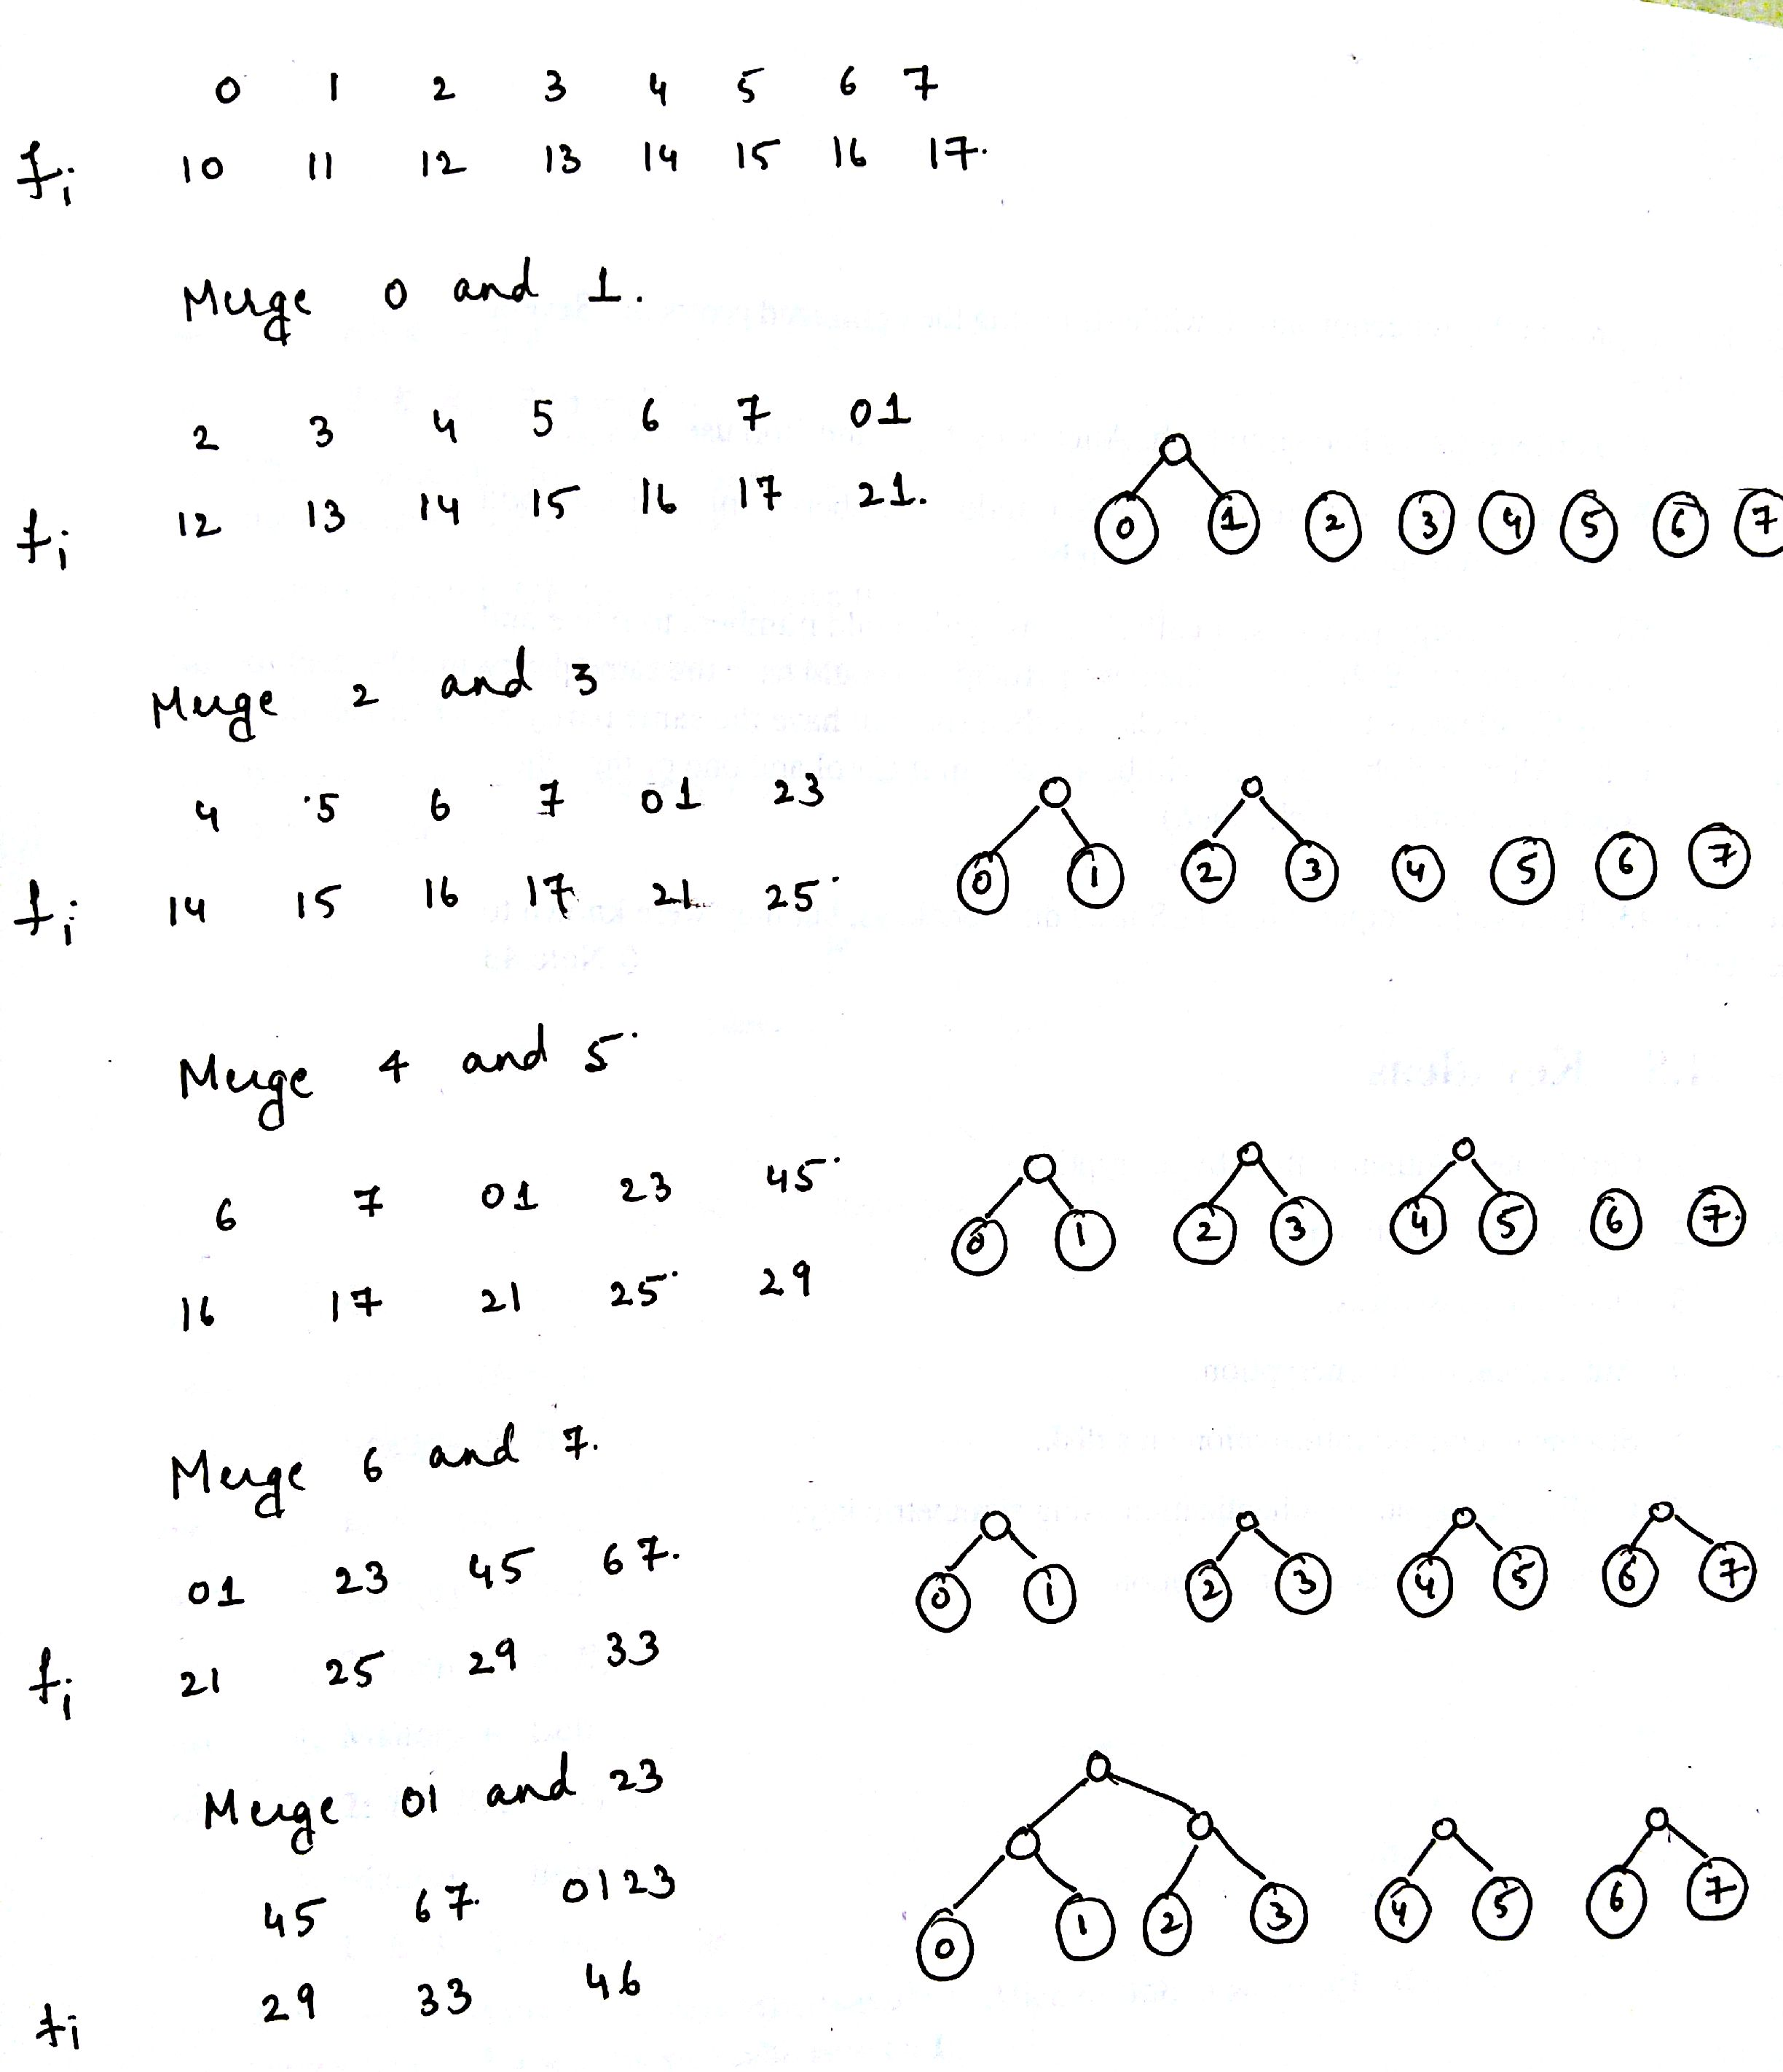
\includegraphics[width=0.8\columnwidth]{a1.jpg}
\end{figure}

\begin{figure}[H]
	\centering
	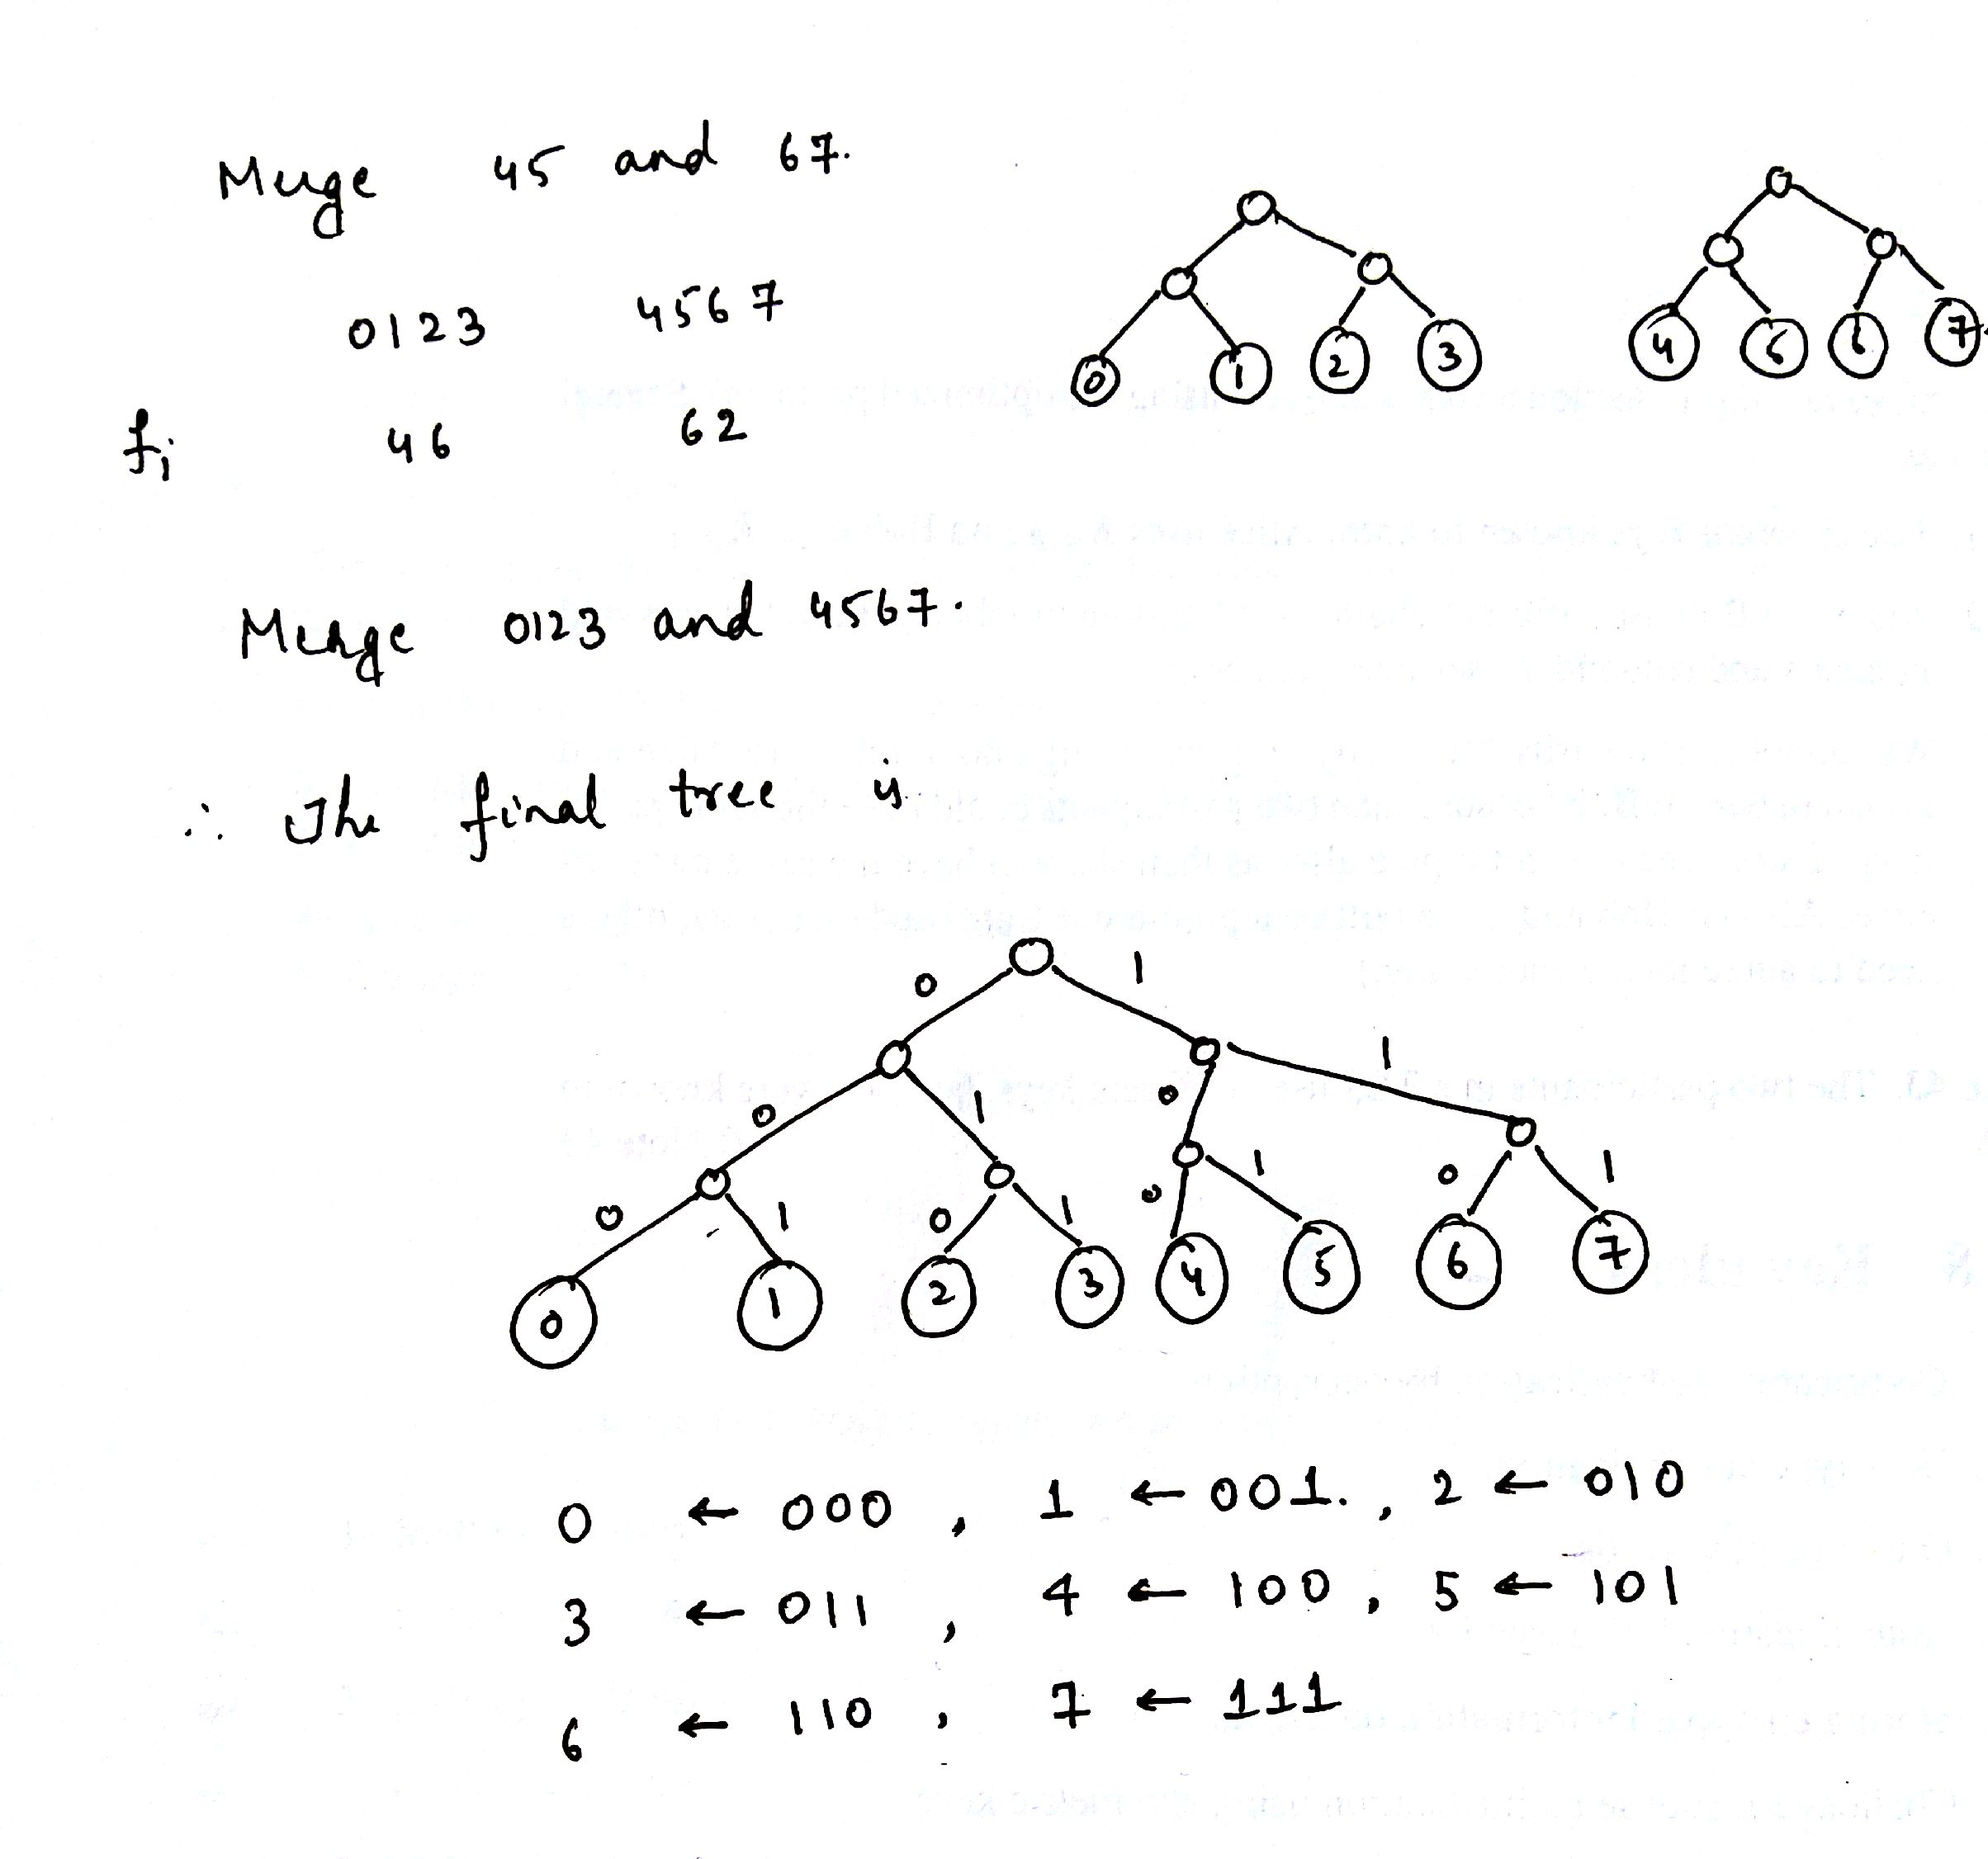
\includegraphics[width=0.8\columnwidth]{a2.jpg}
\end{figure}
\end{solution}
\fi
\pagebreak
\item[(b)] (4 pts) Geometric: $f_i = 10\cdot 2^i$, for $i=0\ldots 7$.

\ifnum\me<2
\begin{solution}
\begin{figure}[H]
	\centering
	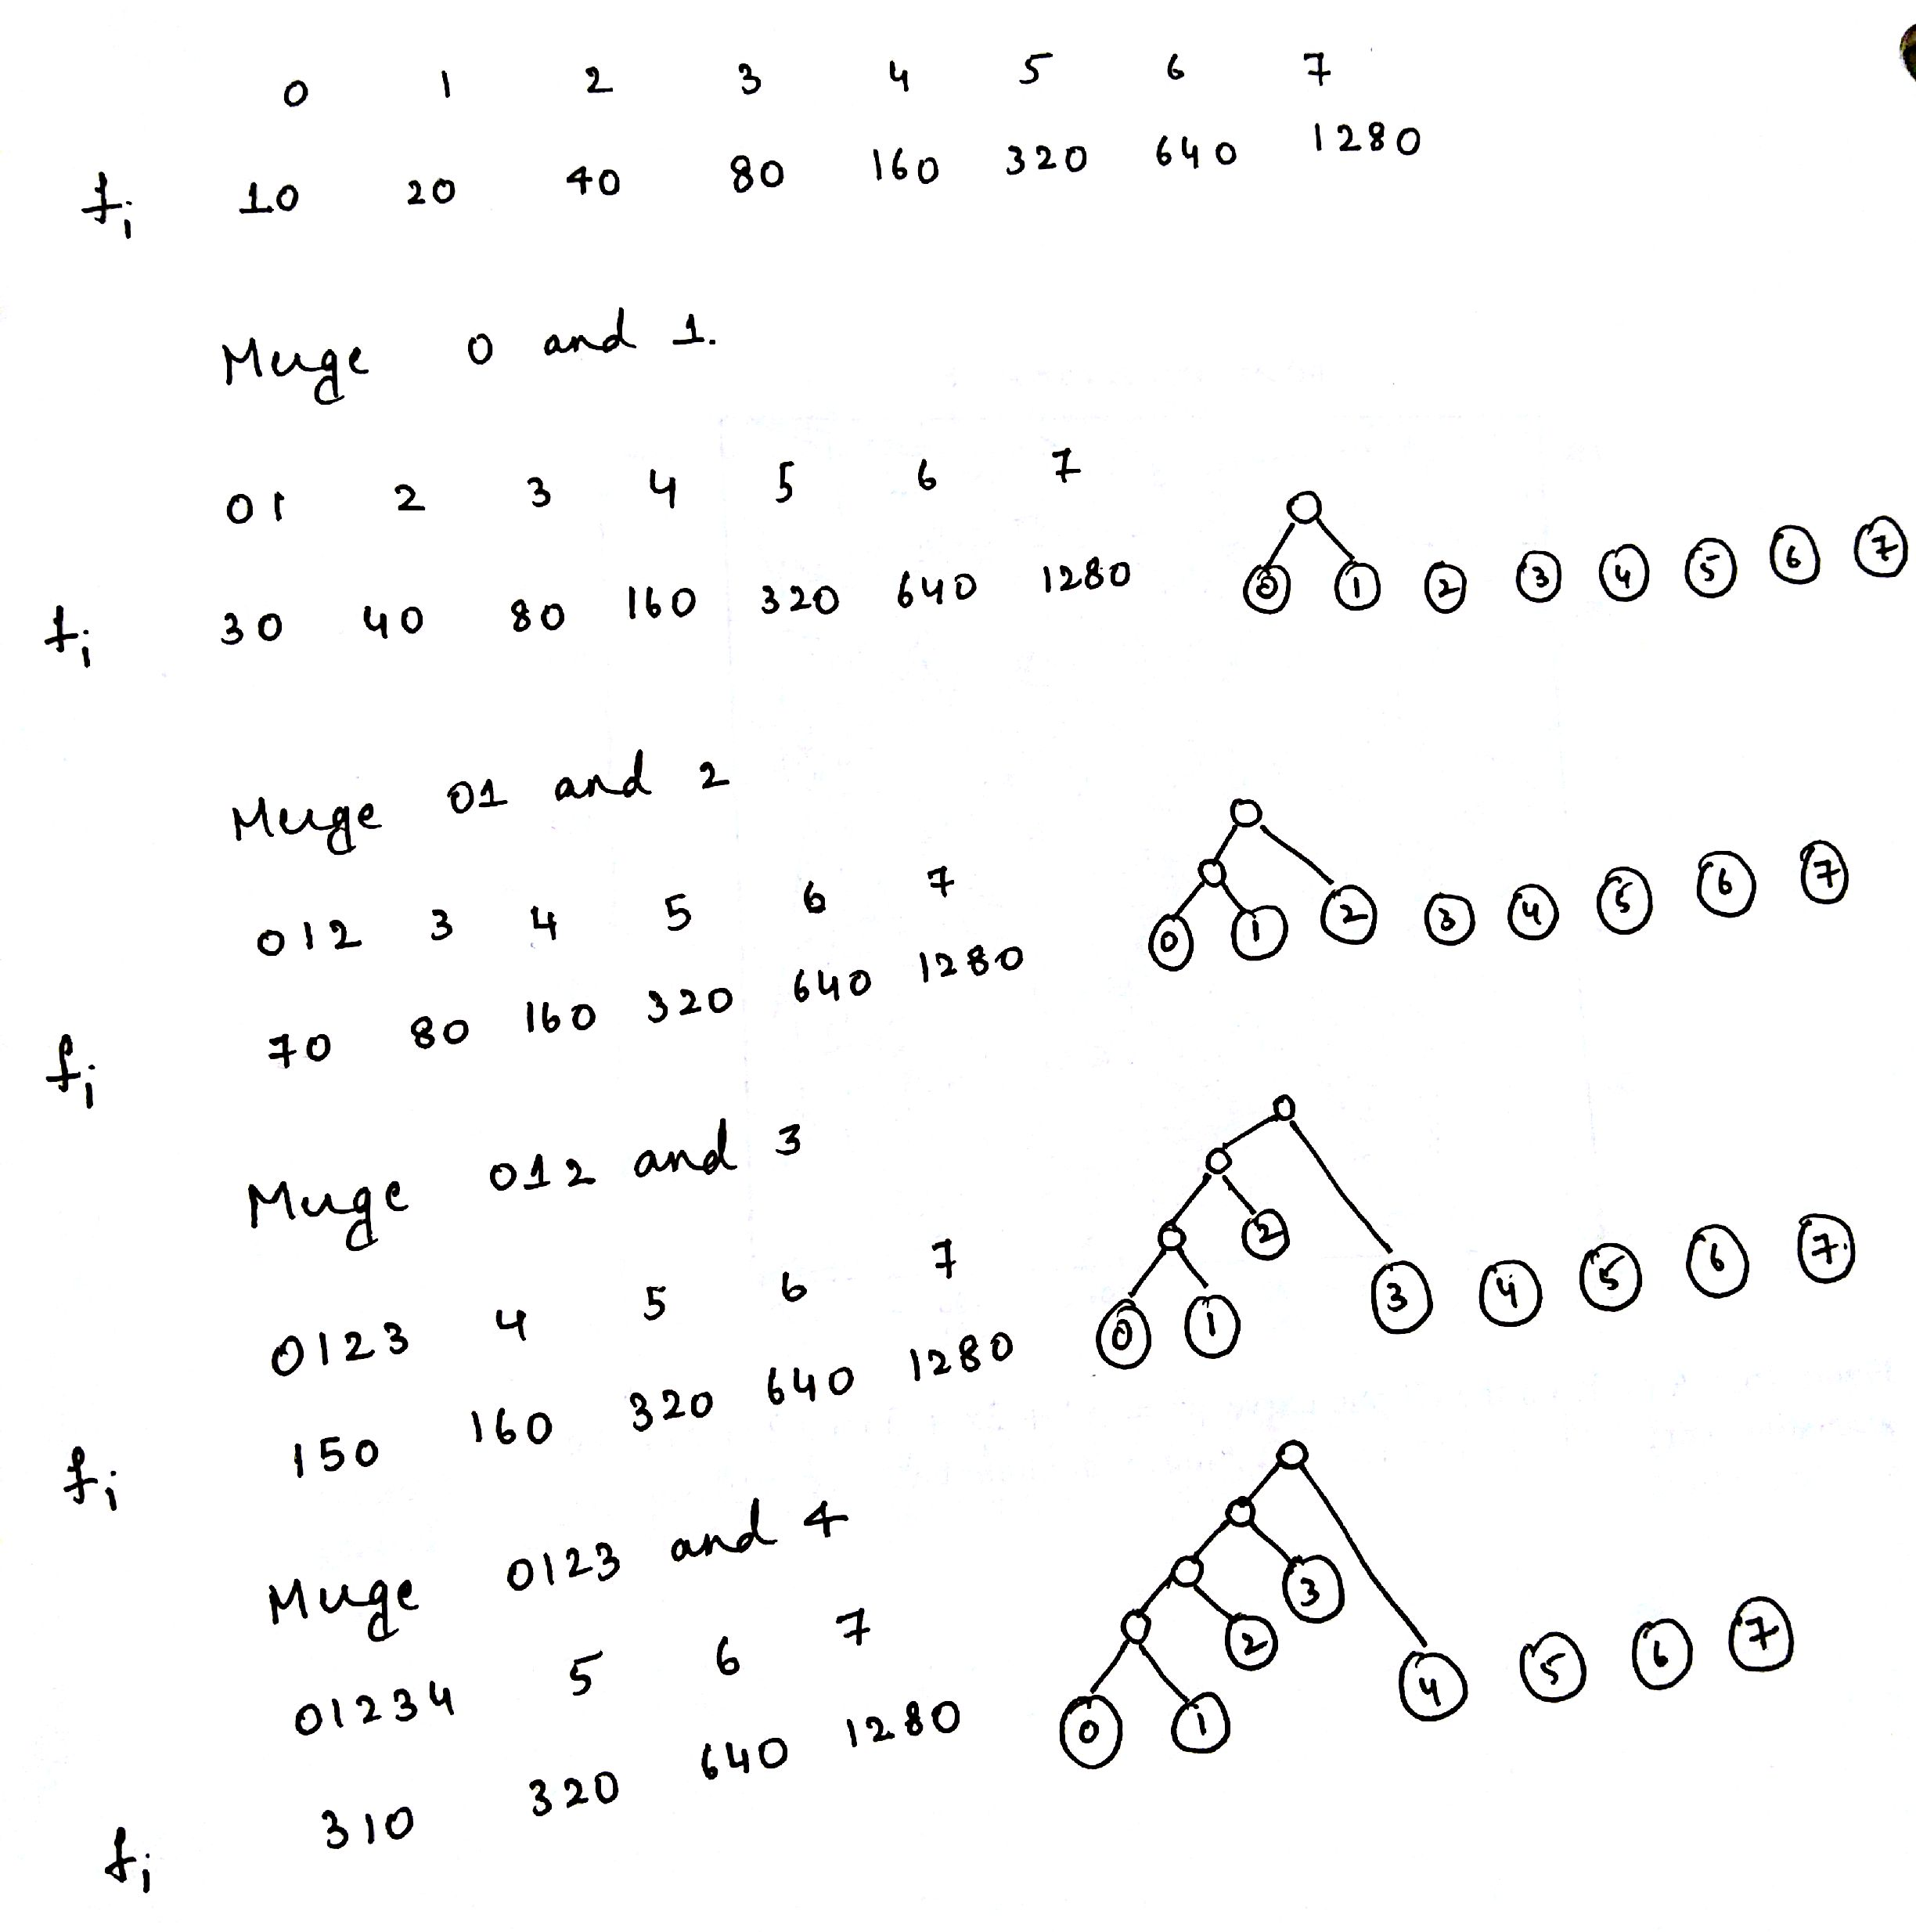
\includegraphics[width=0.8\columnwidth]{b1.jpg}
\end{figure}

\begin{figure}[H]
	\centering
	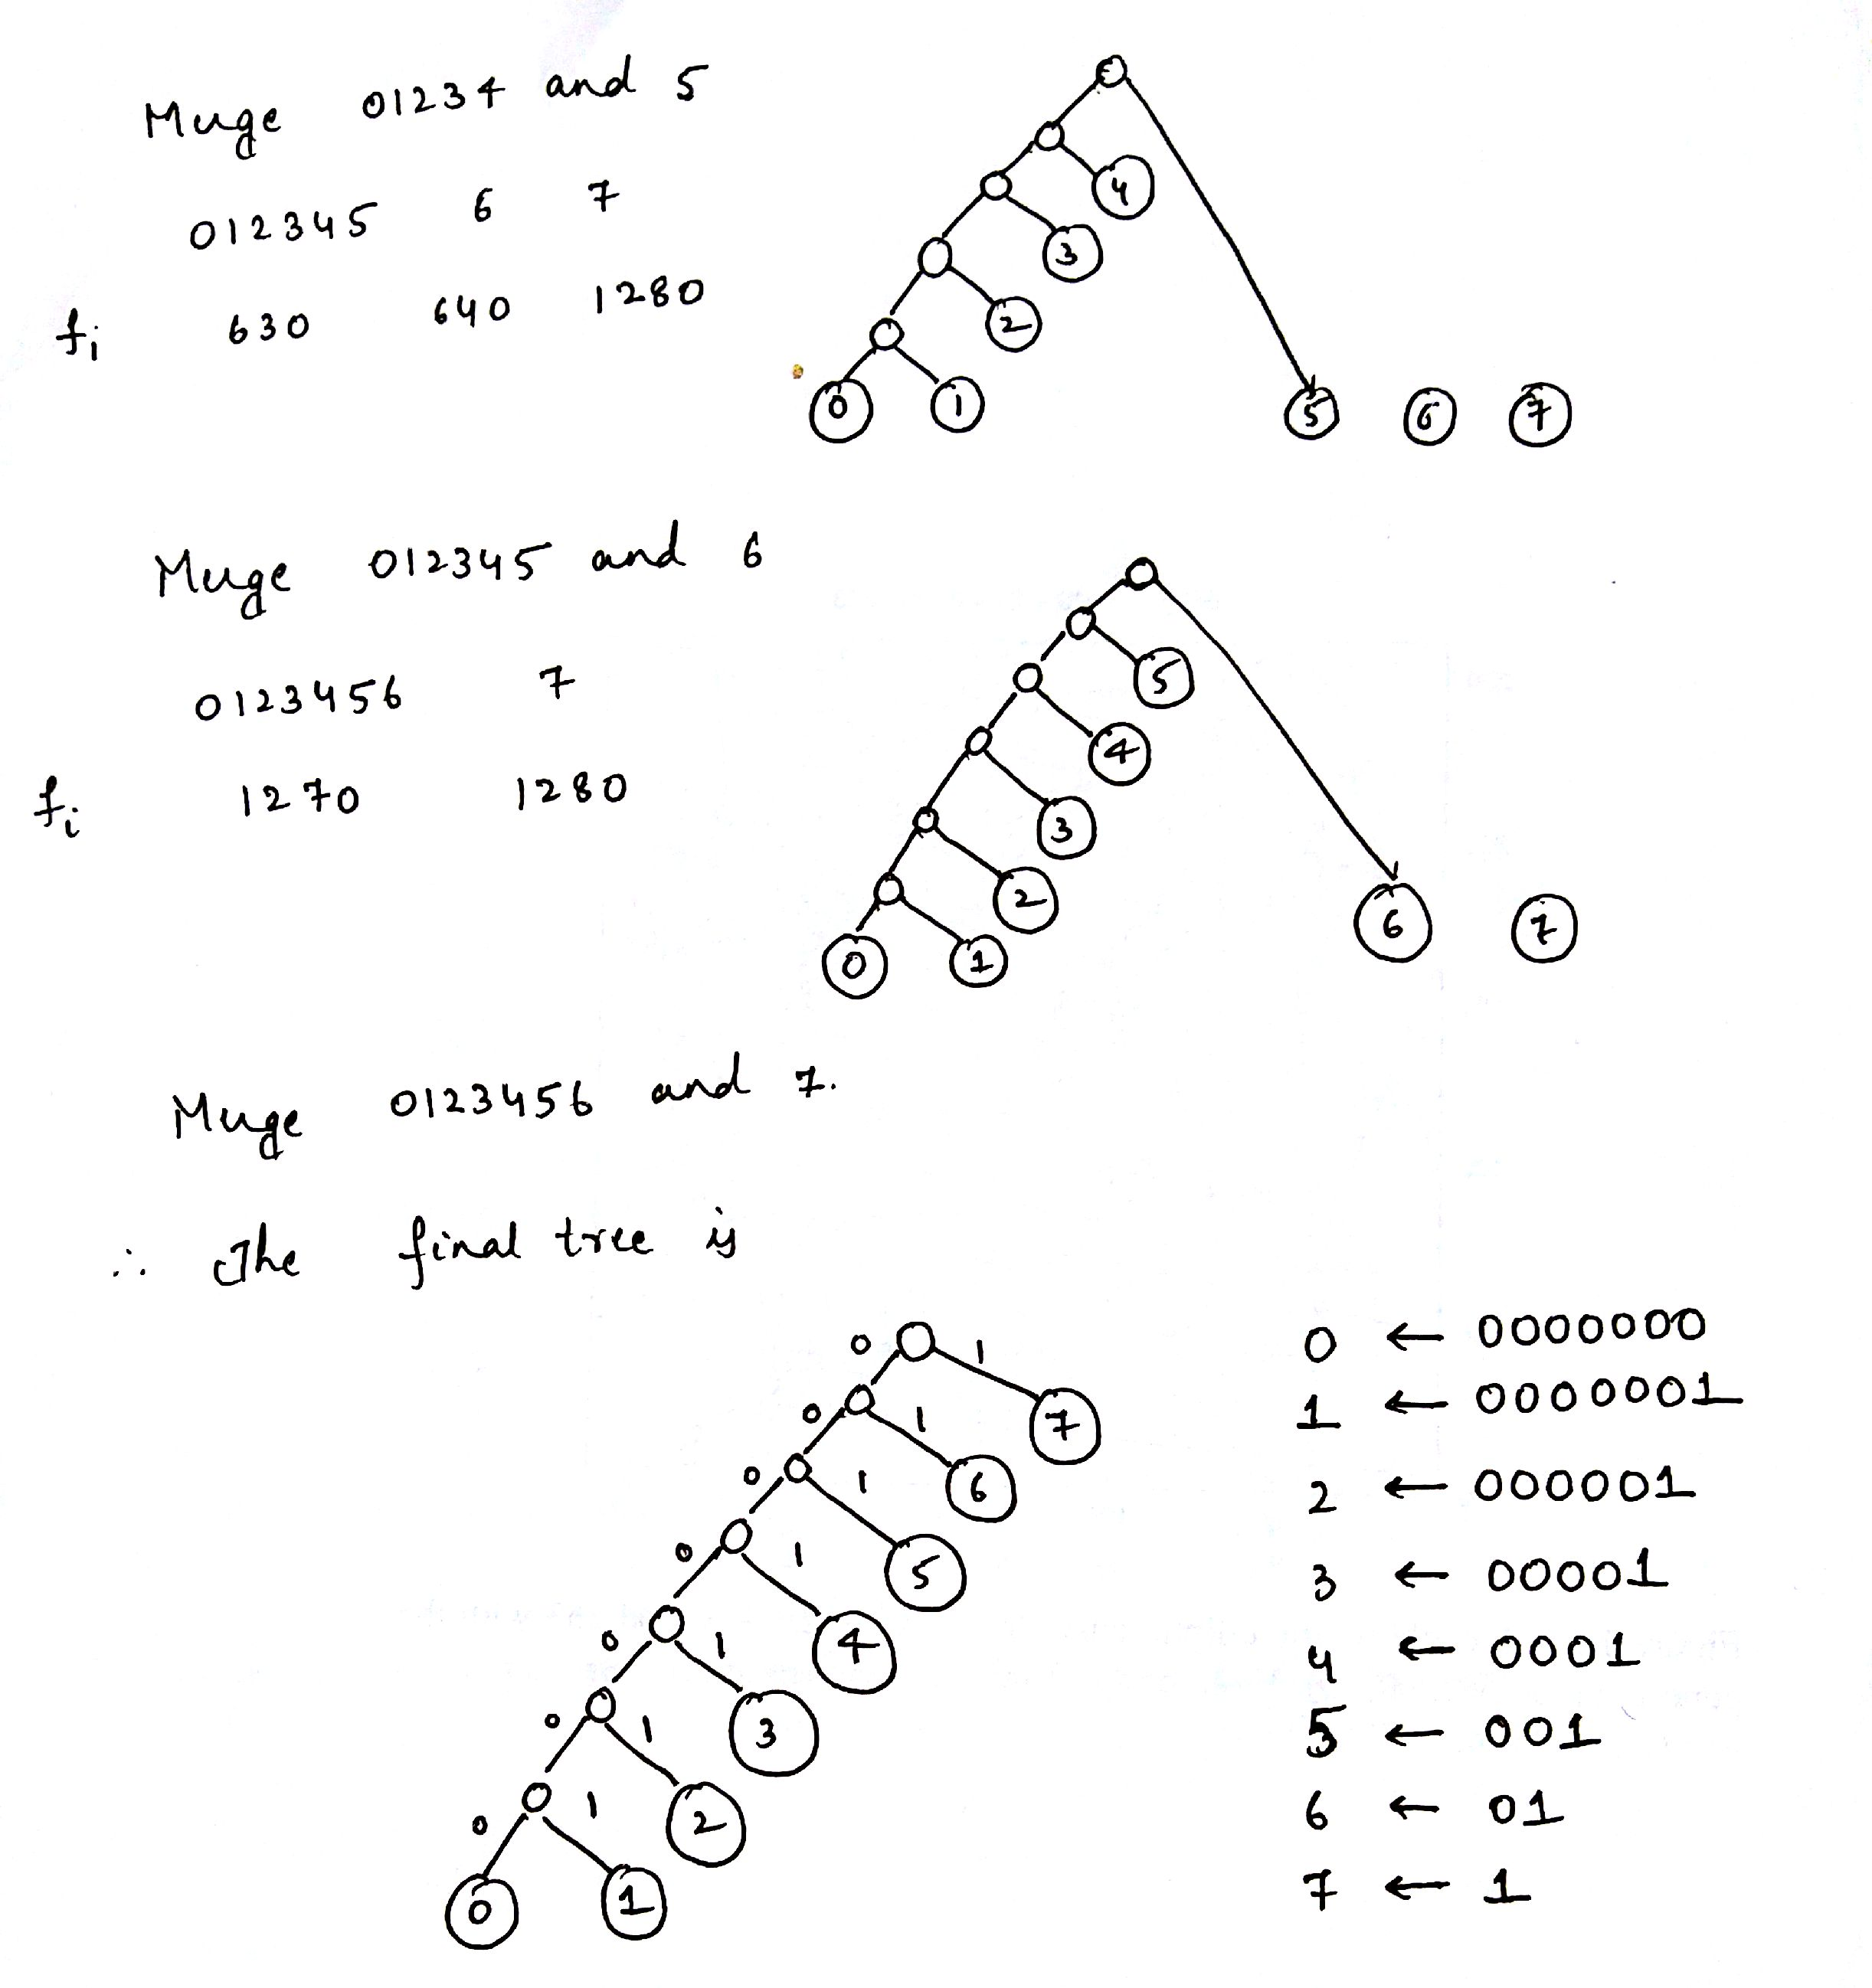
\includegraphics[width=0.8\columnwidth]{b2.jpg}
\end{figure}

The Huffman code for arithmetic is more balanced than that of geometric
\end{solution}
\fi
\end{itemize}


\newproblem{List Merging}{20 Points}



Consider the problem of merging $k$ sorted lists $L_1\ldots L_k$ of
sizes $n_1,\ldots,n_k$, where $n_1+\ldots+n_k=n$. We know that using a
priority queue of size $k$, we can implement this merge it time
$O(n\log k)$ (by repeatedly extracting smallest element from priority
queue and replacing it by the next element of the list it came from).

Here we will design an alternative algorithm which repeatedly finds
two sorted lists and merges them, so that after $k-1$ merges of two
lists we are left with a single sorted list. Assume merging two lists
of size $\ell_1$ and $\ell_2$ takes time $\ell_1+\ell_2$ (irrespective
of the actual elements inside the lists). We would like to find the
order of the $k-1$ merges which minimizes the total cost.

E.g., when $k=3$, we have three choices depending on which two lists
we merge first. If we start with $L_1$ and $L_2$ (costing
$n_1+n_2=n-n_3$), and then merge the result with $L_3$ (cost
$(n_1+n_2)+n_3=n$), we pay $(n-n_3)+n = 2n-n_3$. Similarly, if we
start with $L_2$ and $L_3$ (costing $n_2+n_3=n-n_1$), and then merge
the result with $L_1$ (cost $(n_2+n_3)+n_1=n$), we pay $(n-n_1)+n =
2n-n_1$. Finally, if we start with $L_1$ and $L_3$ (costing
$n_1+n_3=n-n_2$), and then merge the result with $L_2$ (cost
$(n_1+n_3)+n_2=n$), we pay $(n-n_2)+n = 2n-n_2$. Thus, the best cost
achievable is $\min(2n-n-1,2n-n_2,2n-n_3) = 2n -\max(n_1,n_2,n_3)$,
which means the we should exclude the largest list from the first
merge (i.e., merge the two smallest lists first).

\begin{itemize}

\item[(a)] (4 pts) The first (naive) hope is that the order of the merges does not
matter ``too much''. For any $k<n$, given an example of $k$ inputs
$n_1\ldots n_k$ summing to $n$, and a really poor choice of the merge
order, so that the total cost of the merges is $\Theta(nk)$. I.e., for
$k>\log n$ this is much worse than simply sorting the $n$ total
numbers from scratch!

\ifnum\me<2
\begin{solution}

Let $k=8$ and $n_1=1, n_2=2, n_3=3, n_4=4,n_5=5, n_6=6,n_7=7, n_8=8 \implies n = 36, k > \log n$. Merge lists in the descending order i.e start merging $n_8$ with $n_7$ then with $n_6$ and so on. Therefore the total cost of merging these $k$ lists will be $(15+21+26+30+33+35+36) = 196 = \Theta(nk)$ 
\end{solution}
\fi

\item[(b)] (4 pts) Represent any valid order of $(k-1)$ merges as a binary
tree, where the $k$ leaves are labeled by the $k$ initial lists with
sizes $n_1\ldots n_k$, and every merge of two lists corresponds to
creating a parent node of size equal to the sum of the two lists
(children) just merged. Given a particular tree (i.e., order of
merges), write the total cost of all the merges as a function of
$n_1\ldots n_k$ and the depths $d_1\ldots d_k$ of the initial $k$
lists (leaves) in this tree.

\ifnum\me<2
\begin{solution}

Without loss of generality assume that the merge order is $n_1,n_2,n_3, \ldots, n_k$. In the first step when $n_1, n_2$ are merged, the cost is $n_1+n_2$. Now we have a new list of size $n_1+n_2$ that will be merged with $n_3$. So the total cost until now is $(n_1+n_2)+(n_1+n_2+n_3)$. After $k-1$ merges the the cost will be  $(n_1+n_2)+(n_1+n_2+n_3)+ \ldots+ (n_1+n_2+\ldots+n_k)$.Notice that $n_i$ would have occurred exactly $d_i$ times in this summation. Therefore the total cost of merging these $k$ lists will be $\sum_{i=1}^{k}n_id_i$ 
\end{solution}
\fi

\item[(c)] (4 pts) Consider the Huffman code problem with $k$ characters
$c_1\ldots c_k$, where frequency of $c_i$ is $f_i = n_i/n$.  Using
part (b), argue that the optimal tree (order or merges) for the list
merging problem is {\em identical} to the optimal tree (i.e.,
prefix-free code) for the Huffman code problem.

\ifnum\me<2
\begin{solution}

In the optimal tree for the Huffman code, first we merge the two characters with the least frequencies from all the given set of characters i.e if $c_k, c_p$ are the first two characters to be merged then $f_k \leq f_p < \ldots = n_k \leq n_p < \ldots$ and then form a new alphabet $c_{kp}$ whose frequency is $f_k+f_p$ and add this new alphabet to the existing set of alphabets. 

In the optimal tree for the merging problem, first we merge the two lists with the least number of elements from all the given set of lists i.e if $L_k, L_p$ are the first two lists to be merged then $n_k \leq n_p < \ldots$ and then form a new list $L_{kp}$ whose size is $n_k+n_p$ and add this new list to the existing set of lists.

So there is a one to one correspondence between these two problems, therefore the optimal tree for the list merging problem is identical to the optimal tree for the Huffman code problem 
\end{solution}
\fi

\item[(d)] (4 pts) Based on part (c), develop an optimal greedy algorithm for
the list merging problem. Express the running time of the list merging
solution (not just determining the order or merges, but also the
merges themselves!) as the function of $n,k$ and $V$, where $V$ is the
optimal solution {\em value} for the Huffman code problem introduced
in part (b). Do not forget to count the time use to actually solve the
Huffman code problem!

\ifnum\me<2
\begin{solution}

Maintain a pointer for every leaf node to it's corresponding array and when any two leaf nodes are merged into a single node, this merged node contains a pointer to the merged array.

Proceeding this way up until the root, we finally get the resulting list formed by merging all the given $k$ lists. This is identical to Huffman code problem and additionally at every step we are also merging two lists. Therefore the running time will be running time of Huffman code problem (with $k$ leaf nodes = $k \log k$) and time taken to merge all the $k$ lists

From part(b), we know that the cost of all the merges is $\sum_{i=1}^{k} n_id_i = n\sum_{i=1}^{k} f_id_i = nV$ where $V = \sum_{i=1}^{k} f_id_i$. Hence the total running time is $O(k \log k + nV)$
\end{solution}
\fi
\pagebreak
\item[(e)] (4 pts) Prove that $V\le \log k$ (think of one solution which is
always an option),\footnote{It turns out that one can prove a much
tighter bound on $V$: $V\in [H,H+1]$, where $H = \sum_{i=1}^k
\frac{n_i}{n} \log_2(\frac{n}{n_i})$ is called the {\em entropy} of
the probability distribution
$(\frac{n_1}{n},\ldots,\frac{n_k}{n})$. Moreover, for many ``skewed''
distribution, $H,V\ll \log k$.}  and substitute $V=\log k$ into the
formula you got in part (d). How does it compare with the original
$O(n\log k)$ solution?

\ifnum\me<2
\begin{solution}

If the tree is a perfectly balanced binary tree then $d_i= \log k \,\,\, \forall i = 1$ to $k \\\implies V = \frac{1}{n} \sum_{i=1}^{k} n_id_i = \frac{\log k}{n} \sum_{i=1}^{k} n_i = \log k$

If the tree is not perfectly balanced i.e like the tree in Problem-3, part(b), i.e $d_i = i$, then $V = \frac{1}{n} \sum_{i=1}^{k} n_id_i = \frac{1}{n} \sum_{i=1}^{k} n_ii \leq \log k$.

Therefore $V \leq \log k$. Substitute this value of $V$ in part (d), we get the running time\\ $T(n) = O(k \log k + n \log k) = O(n \log k)$ i.e the greedy algorithm is not asymptotically significant than the original solution
\end{solution}
\fi

\end{itemize}
\end{document}


